
%%\include{Begin}

\section{バス内(行き)}

\begin{tabular}{p{2zw}rp{38zw}}
  日時 & : & 2019年4月5日(金) 12:10 $\sim$ 14:40\\ %未定
  場所 & : & バス
\end{tabular}

\subsection{目的}
新入生の緊張をほぐし,仲を深める.


\subsection{タイムスケジュール}
% 時刻は必ず4桁(00:00)で書くこと!!!
\begin{longtable}{p{3zw}p{39zw}}
  12:20 & \textbf{◎ バス出発(2号車)} \\
        & \ \ \textbullet \ \ 連絡係(吉田,石野,江川)は受付との乗車チェックが終わり次第,乗車チェックが完了したことを報告LINEに連絡する \\
        & \ \ \textbullet \ \ 全車の乗車チェックが終わり次第,出発する\\
        & \ \ \textbullet \ \ 連絡係はバスが出発したことを報告LINEに連絡する \\
	& \ \ \textbullet \ \ 連絡係はバスの状況を見て話し始める \\\\

  12:22 & \textbf{◎ 司会者挨拶,自己紹介} \\
        & \ \ \textbullet \ \ 司会が新入生と教職員に向けて挨拶する  \\
        & \ \ \textbullet \ \ 司会の自己紹介をする  \\\\
        
  説明しない可能性あり
  12:25 & \textbf{◎これからの流れ説明 } \\
       & \ \ \textbullet \ \ これからのスケジュールを説明する \\\\

  12:27 & \textbf{◎ バス内諸注意,スタッフ紹介} \\
        & \ \ \textbullet \ \ 飲食・ゴミについて説明する\\
        & \ \ \textbullet \ \ 気分の悪い人の対応について説明する\\
        & \ \ \textbullet \ \ 前から順に同席スタッフの紹介をする  \\
        & \ \ \textbullet \ \ その他注意事項があれば説明する  \\\\
        
  12:32 & \textbf{◎ 流れ説明} \\
	& \ \  \textbullet \ \ 到着予定時刻を伝える\\
	& \ \  \textbullet \ \ 到着後の流れを説明する\\\\

 12:40 & \textbf{◎ 道の駅(風良里)到着5分前} \\
	& \ \  \textbullet \ \ もうすぐ道の駅(風良里)に到着する連絡と,トイレの場所,出発時間 5 分前にバス内に着席することを新入生に説明する\\
        & \ \  \textbullet \ \ 休憩時間は10分\\\\
        
 12:45 & \textbf{◎ 道の駅(風良里)到着} \\
	& \ \  \textbullet \ \ 補助席に座ってる人が先に降りる\\
	& \ \  \textbullet \ \ スタッフは新入生の奇行に目を配る\\
	& \ \  \textbullet \ \ バス連絡係はスラックで到着の旨を連絡する \\\\

12:55 & \textbf{◎ 乗車開始} \\
	& \ \  \textbullet \ \ 気分が悪い人がいないか確認する(もしいた場合は救護車に移動してもらう)\\
	& \ \  \textbullet \ \ 司会者は新入生に隣の席の人がいるか確認してもらい,人数を確認する\\
	& \ \  \textbullet \ \ バス連絡係はバス司会LINEで乗車開始の旨を連絡する\\\\

13:00 & \textbf{◎ 道の駅(風良里)出発} \\
	& \ \  \textbullet \ \ 運転手に乗車確認を伝え順次出発する\\
	& \ \  \textbullet \ \ バス連絡係は報告LINEで出発の旨を連絡する\\\\

13:05  & \textbf{◎ 教員紹介} \\ 
	& \ \ \textbullet \ \ 教員を紹介する(しゃべる内容をある程度指定しておく)\\
	& \ \ \textbullet \ \ 幡多でも自己紹介はあるので,長くならず固くならない程度にしゃべってもらう  \\\\
	
13:10 & \textbf{◎ バス内企画 その1} \\
      	& \ \  \textbullet \ \ 自己紹介\\
        & \ \ \ \ \  - 自己紹介カードを用いて隣の人と自己紹介を行う\\
        & \ \ \ \ \  - まれに,となりの人がいないときがあるため,その場合はスタッフと自己紹介する\\\\
	% いるかどうかわからないので一応コメント化 用途が分かり次第変更
        % & \ \ \textbullet \ \ 方言当てゲーム, お題あてゲーム, 連想ゲーム, 心理テスト, 100分の1ゲーム \\
        % & \ \ \ \ \ - ルール説明 \\
        %       & \ \ \ \ \ - ゲーム \\
        % & \ \ \ \ \ - 商品をプレゼント \\
        % & \ \ \ \ \ - ?安芸駅に到着するまでに質問がでなかった場合1人に近い質問をした人に商品をプレゼントする.\\\\

13:25 & \textbf{◎ バス内企画 その2} \\
	& \ \  \textbullet \ \ 方言当てゲーム\\
  & \ \ \ \ \ - 各地方の珍しい方言を当ててもらう. \\
  & \ \ \ \ \ - フリートークの際などに,   各々の出身地の方言などで新入生同士が盛り上がれるよう司会が流れを作る.\\\\
  
 13:55 & \textbf{◎ あぐり窪川到着5分前} \\
	& \ \  \textbullet \ \ もうすぐあぐり窪川に到着する連絡と,トイレの場所,お店の利用について,   出発時間 5 分前にバス内に着席することを新入生に説明する\\
        & \ \  \textbullet \ \ 休憩時間は25分\\\\
        
 14:00 & \textbf{◎ あぐり窪川到着} \\
	& \ \  \textbullet \ \ 補助席に座ってる人が先に降りる\\
	& \ \  \textbullet \ \ スタッフは新入生の奇行に目を配る\\
	& \ \  \textbullet \ \ バス連絡係はスラックで到着の旨を連絡する \\\\

14:25 & \textbf{◎ 乗車開始} \\
	& \ \  \textbullet \ \ 気分が悪い人がいないか確認する(もしいた場合は救護車に移動してもらう)\\
	& \ \  \textbullet \ \ 司会者は新入生に隣の席の人がいるか確認してもらい,人数を確認する\\
	& \ \  \textbullet \ \ バス連絡係はバス司会LINEで乗車開始の旨を連絡する\\\\

14:30 & \textbf{◎ あぐり窪川出発} \\
	& \ \  \textbullet \ \ 運転手に乗車確認を伝え順次出発する\\
	& \ \  \textbullet \ \ バス連絡係は報告LINEで出発の旨を連絡する\\\\

14:35 & \textbf{◎ バス内企画 その3} \\
	& \ \  \textbullet \ \ 100分の1ゲーム\\
  & \ \ \ \ \ - バス内で1人だけのお題を考えてもらう.   見事1人だけ当てれたら景品(スパイス)をプレゼント.  \\
  & \ \ \ \ \ - 野外炊事で景品が使えることをさりげなく説明,   新入生が周りとコミュニケーションを取りやすくなる.\\\\
  
15:10 & \textbf{◎ 幡多到着5分前} \\
	& \ \  \textbullet \ \ タイムライン上は到着5分前だが本番は山道に入ったところでもうすぐ着くというアナウンスをする\\
        & \ \  \textbullet \ \ 名札をつけていることを確認してもらい,野外炊事のグループを名札で確認をしてもらう\\
        & \ \  \textbullet \ \ トイレ,荷物について説明する\\
        & \ \  \textbullet \ \ 入所式の並び方を説明する\\
	& \ \  \textbullet \ \ バス連絡係は報告LINEで山道に入った旨を連絡する\\\\

15:15 & \textbf{◎ 幡多到着} \\
& \ \ \textbullet \ \ 到着後スタッフは速やかに降りて荷下ろしをする\\
	& \ \ \textbullet \ \ 3号車は2号車の荷下ろしの手伝いをする \\
	& \ \ \textbullet \ \ 道の駅(風良里)とあぐり窪川の休憩とは違い全員がバスから降りるので前から順に速やかに降りてもらう\\
        & \ \ \textbullet \ \ 到着した旨を報告LINEに連絡する\\\\
\end{longtable}

%%\subsection{内容}
\subsection{人員配置(図\ref{fig:bus_memberHaichi1},\ref{fig:bus_memberHaichi2},参照)}
○1号車
\begin{itemize}
\item 司会:藤田,北村
\item 補助: 
\end{itemize}
○2号車
\begin{itemize}
\item 司会:中島,高橋
\item 補助:

\end{itemize}
○3号車
\begin{itemize}
\item 司会:丸田,塩谷
\item 補助:

\end{itemize}


\subsection{トランク内荷物配置図}
\begin{figure}[H]
  \begin{tabular}{lr}
    \begin{minipage}{0.5\textwidth}
  \begin{center}
  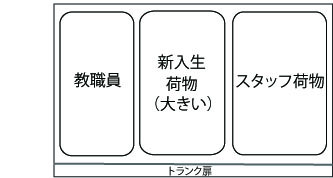
\includegraphics[width=8cm]{./06/baggage_place_1.eps}
  \caption{トランク内荷物配置図(1号車)}
\end{center}
\end{minipage}

\begin{minipage}{0.5\textwidth}
\begin{center}
  \includegraphics[width=8cm]{./06/baggage_place_2.eps}
  \caption{トランク内荷物配置図(2号車)}
\end{center}
\end{minipage}
\end{tabular}
\end{figure}


\subsection{必要物品}
\begin{itemize}
\item 酔い止め薬:各バス1箱
\item エチケット袋:各バス2枚
\item 紙コップ:各バス5個
\item 水(常温):各バス500ml(1本)
\item キッチンタイマー
\item 100分の1ゲームの商品:野外炊事に使用する調味料3種類*3セット
\end{itemize}

\subsection{備考}

\begin{itemize}
\item 司会のどちらが報告LINEに連絡を入れるか,各号車ごとに事前に決めておく
\item 先遣隊,他のバス,後遣隊等と随時連絡を取り合う
\item 新入生の体調確認を忘れない
\end{itemize}


%%\include{End}
